\documentclass{article}
\usepackage[utf8]{inputenc}
\usepackage{amsmath}
\usepackage{tikz}
\usetikzlibrary{trees}

\title{LaTeX Test Document}
\author{Your Name}
\date{\today}

\begin{document}

\maketitle

\section{Introduction}
This is a test document to verify your LaTeX setup is working correctly.

\section{Math Example}
Here's a simple equation:
\begin{equation}
    E = mc^2
\end{equation}

And an inline equation: $x = \frac{-b \pm \sqrt{b^2 - 4ac}}{2a}$

\section{Tree Example}
Here's a simple tree using TikZ:

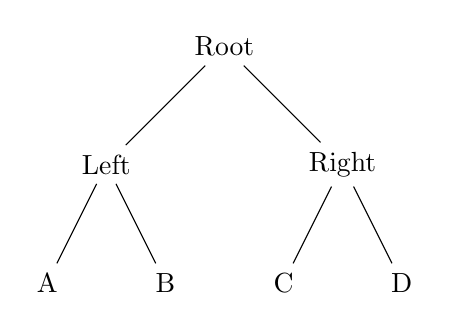
\begin{tikzpicture}[level distance=1.5cm,
  level 1/.style={sibling distance=3cm},
  level 2/.style={sibling distance=1.5cm}]
  \node {Root}
    child {node {Left}
      child {node {A}}
      child {node {B}}
    }
    child {node {Right}
      child {node {C}}
      child {node {D}}
    };
\end{tikzpicture}

\section{List Example}
\begin{itemize}
    \item First item
    \item Second item
    \item Third item
\end{itemize}

\section{Conclusion}
If this compiles and displays correctly, your LaTeX environment is working!

\end{document}
